\documentclass[11pt,a4wide]{article}
\usepackage{verbatim}
\usepackage{listings}
\usepackage{graphicx}
\usepackage{a4wide}
\usepackage{color}
\usepackage[options]{SIunits}
\usepackage{amsmath}
\usepackage{amssymb}
\usepackage[dvips]{epsfig}
\usepackage[utf8]{inputenc}
\usepackage[OT1]{fontenc}
\usepackage{cite} % [2,3,4] --> [2--4]
\usepackage{shadow}
\usepackage{hyperref}

\setcounter{tocdepth}{2}
%
\lstset{language=c++}
\lstset{alsolanguage=[90]Fortran}
\lstset{basicstyle=\small}
\lstset{backgroundcolor=\color{white}}
\lstset{frame=single}
\lstset{stringstyle=\ttfamily}
\lstset{keywordstyle=\color{red}\bfseries}
\lstset{commentstyle=\itshape\color{blue}}
\lstset{showspaces=false}
\lstset{showstringspaces=false}
\lstset{showtabs=false}
\lstset{breaklines}

\begin{document}
\title{report on project solar system}
\author{Ekaterina Ilin and Isabelle Gauger\\GitHub: \url{https://github.com/CPekaterina/Solar-System}
}
\maketitle
\tableofcontents
\newpage
\section{Teilaufgabe d}

We now consider a planet that has the same distance from the sun than earth and want to find out what initial velocity it at least must have to escape from the sun. By trial and error we find an escape velocity of $8.9\frac{\text{AU}}{\text{year}}$ what is $42332.6\frac{\text{m}}{\text{s}}$. At the starting time $t1$ our planet has the velocity $v$ and the distance $r$ from the sun. So it's total energy is given by

\begin{equation}
E_{total}\left(t_1\right) = E_{kin}\left(t_1\right) + E_{pot}\left(t_1\right) = \frac{1}{2}m_{p}v^2 - \frac{Gm_{s}m_{p}}{r}
\end{equation}

We choose $t_2$ as a later point in time when our planet is far away from the sun. The total energy of our planet is than

\begin{equation}
E_{total}\left(t_2\right) = E_{kin}\left(t_2\right) + E_{pot}\left(t_2\right) 
\end{equation}

For $r\rightarrow\infty$ the potential energy of our planet is zero. Our aim is to find the minimum velocity with which our planet escapes out of the sun's gravitational field so we also set the kinetic energy to zero for $t_2$. The total energy has to be preserved what leads to

\begin{equation}
E_{kin}\left(t_1\right) + E_{pot}\left(t_1\right) = E_{kin}\left(t_2\right) + E_{pot}\left(t_2\right) = 0
\end{equation}

what is equal to 

\begin{equation}
\frac{1}{2}m_{p}v^2 - \frac{Gm_{s}m_{p}}{r} = 0
\end{equation}

We rearrange that and get the escape velocity

\begin{equation} 
v=\sqrt{\frac{2Gm_{s}}{r}}=\sqrt{\frac{2*6,67*10^{-11}\frac{\text{m}^3}{\text{kg}\text{s}^2}*2*10^{30}\text{kg}}{1,5*10^{11}\text{m}}}=42174.2\frac{\text{m}}{\text{s}}
\end{equation}

The value we get for the escape velocity by trial and error is around the exact solution, but of course not very precise.  

\section{Teilaufgabe e}
We now include Jupiter (see http://en.wikipedia.org/wiki/Jupiter) in our system. The trajectories of Earth and Jupiter calculated with the fourth-order Runge-Kutta method are shown in figure \ref{fig:Earth and Jupiter XY}. To find out for which timesteps $h$ the solutions calculated with Verlet and RK$4$ are stable we calculated the positions of Earth and Jupiter for different values of $h$ and a time of $1000$ years. We found that with the Verlet algorithm the solution for Earth is stable for $h\le 0.16$ and the solution for Jupiter for $h\le 2.01$. When we divide these values through the respective orbital period we see that the Verlet method is stable for $h$ around a sixth of the orbital period or smaller. For RK$4$ we found that the solution for Earth is stable for $h\le 0.03$ and the solution for Jupiter for $h\le 0.68$. We see that an advantage of the Verlet algorithm is that it is stable for larger timesteps than the RK$4$ method. 

\begin{figure}
\centering
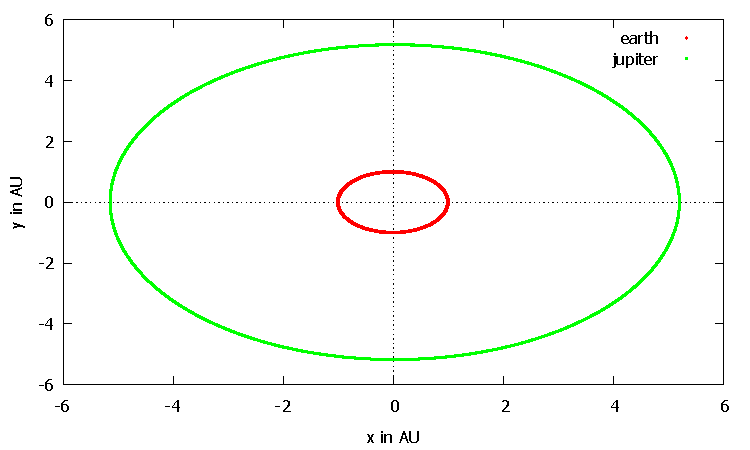
\includegraphics[scale=0.45]{jupiter_earthXY.pdf}
\caption{The trajectories of Earth and Jupiter calculated with RK$4$}
\label{fig:Earth and Jupiter XY}
\end{figure}  

In the next step we increase the mass of Jupiter by a factor of $10$ and repeat the calculations. The position of Earth is shown in figure \ref{fig:EarthXY 10x}. The solution for Earth calculated with the Verlet method is still stable for $h\le0.16$ and with the RK$4$ method it is stable for $h\le 0.02$. The increase of Jupiter's mass by a factor of $10$ causes nearly no change when we look at the solution for Earth and it's stability. When we increase the mass of Jupiter by a factor of $1000$ this is totally different. Figure \ref{fig:EarthXY 1000x} shows the position of Earth calculated with RK$4$ for a timestep $h=0.0001$ and a time of $3$ years. We don't get a closed orbit for Earth anymore and even if we choose $h=0.00001$ both algorithms are unstable.

\begin{figure}
\centering
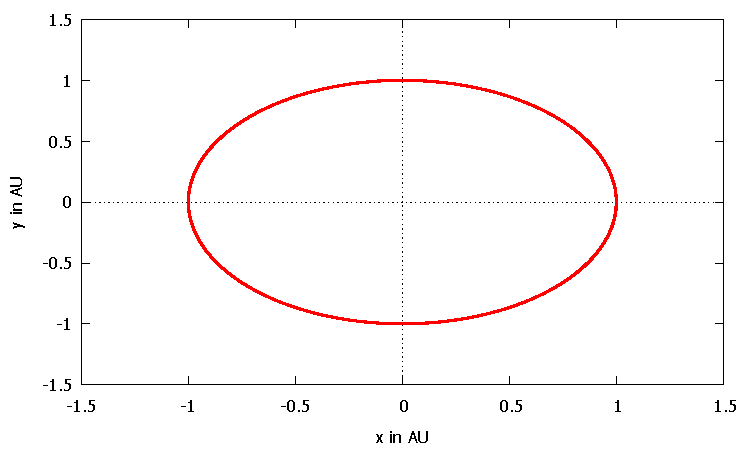
\includegraphics[scale=0.45]{positionEarth10x3a.pdf}
\caption{The trajectory of Earth calculated with RK$4$ for $10$x the normal mass of Jupiter}
\label{fig:EarthXY 10x}
\end{figure}  

\begin{figure}
\centering
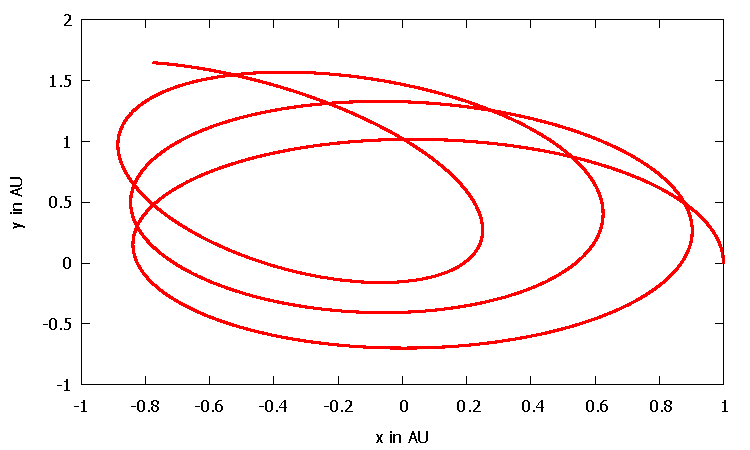
\includegraphics[scale=0.45]{positionEarth1000x3a.pdf}
\caption{The trajectory of Earth calculated with RK$4$ for $1000$x the normal mass of Jupiter}
\label{fig:EarthXY 1000x}
\end{figure} 



\end{document}
   
